\documentclass[12pt,a4paper]{article}
\usepackage[margin=2cm, left=1.5cm, right=1.5cm]{geometry}
\usepackage{amsmath, amssymb, amsthm}
\usepackage{fancyhdr}
\usepackage{mdframed}
\usepackage{enumerate}
\usepackage{graphicx}
\usepackage{float}

\pagestyle{fancy}
\fancyhf{}
\fancyhead[L]{113-1 Machine Learning}
\fancyhead[R]{Final Project}
\fancyfoot[C]{\thepage}
\setlength{\headheight}{15pt}

\usepackage{silence}
\WarningFilter{latexfont}{Font shape}
\WarningFilter{latexfont}{Some font shapes were not available}

\usepackage{xeCJK}
\setCJKmainfont[AutoFakeBold=true, AutoFakeSlant=true]{bkai00mp.ttf}
\setCJKmonofont[AutoFakeBold=true, AutoFakeSlant=true]{bkai00mp.ttf}
\setCJKsansfont[AutoFakeBold=true, AutoFakeSlant=true]{bkai00mp.ttf}

% remove all figures for faster compilation
% \usepackage[allfiguresdraft]{draftfigure}

\linespread{1.25}

\begin{document}
\begin{center}
  {\LARGE \bf HTML 2024 Final Project}\\[8pt]
  \textbf{Team:} How To Make Lasagna\\
  B12902119 胡祐誠 B12902123 常洧丞 B12902037 張聲元 B11902139 洪佑全
\end{center}


\section{Introduction}

\section{Preprocessing}

\section{Model}

\subsection{Logistic Regression}

Logistic regression is the only approach we use that is in the MLF. We expect that it will be the least accurate one, but we still want to see how it performs. We used the preprocessed data to train the model, and split the data into 80\% training and 20\% validation. We trained the model 5000 times and choose the one with the highest validation accuracy for both stage 1 and stage 2. The highest validation accuracy we got in stage 1 was 0.64, and in stage 2 was 0.61. In spite of this, the performance of logistic regression in private was 0.56 in stage 1, and 0.53 in stage 2. Overall, logistic regression is one of the worst models we used in this project.



\subsection{Support Vector Machine}

In this section, we discuss the application of three different Support Vector Machine (SVM) models: linear kernel, polynomial kernel, and Gaussian kernel.


\subsubsection{Linear Kernel}

For the linear kernel SVM, we implemented the model using the \texttt{sklearn.svm.SVC} class and conducted hyperparameter tuning with \texttt{GridSearchCV}. The grid search was performed with 3-fold cross-validation, focusing on two key hyperparameters:
\begin{itemize}
    \item \texttt{C}: [0.1, 1.0, 10]
    \item \texttt{tol}: [1e-3, 1e-4]
\end{itemize}

The best hyperparameters found were \texttt{C} = 10 and \texttt{tol} = 0.001, with a cross-validation accuracy of \textbf{60.57\%}. We use the best hyperparameters and full training data to train the final model.


\paragraph{Kaggle Performance}

The linear kernel SVM scored \textbf{0.55681} (public) and \textbf{0.55296} (private) in Stage 1 of the Kaggle competition. In Stage 2, the scores were \textbf{0.51411} (public) and \textbf{0.52614} (private).


\paragraph{Discussion}

The linear kernel SVM provided decent performance with a validation accuracy of \textbf{63.32\%} after tuning. However, its Kaggle competition scores, particularly in Stage 2, highlight the limitations of this approach. The drop in performance from Stage 1 to Stage 2 suggests that the linear kernel struggled to generalize well to more complex or diverse test data. While the linear kernel offers simplicity and efficiency, it may not capture intricate patterns in the data, making it less competitive compared to more flexible kernels such as polynomial or Gaussian in this particular task.


\subsubsection{Polynomial Kernel}

We experimented with a polynomial kernel SVM, but the results were suboptimal, yielding poor accuracy compared to the linear and Gaussian kernels. Due to its underperformance, the polynomial kernel was not considered for the final submission, and we proceeded directly to testing the Gaussian kernel, which showed more promise.


\subsubsection{Gaussian Kernel}

For the Gaussian kernel SVM, we also utilized the \texttt{sklearn.svm.SVC} class and performed hyperparameter tuning with \texttt{GridSearchCV}. The grid search was conducted using 3-fold cross-validation and focused on the following hyperparameters: \begin{itemize} \item \texttt{C}: [0.1, 1.0, 10] \item \texttt{gamma}: [1e-3, 1e-4, 0.001] \end{itemize}

The best hyperparameters found were \texttt{C} = 10 and \texttt{gamma} = 0.001, with a cross-validation accuracy of \textbf{57.01\%}. We use the best hyperparameters and full training data to train the final model.


\paragraph{Kaggle Performance}

The Gaussian kernel SVM achieved \textbf{0.56294} on the public leaderboard and \textbf{0.57304} on the private leaderboard for Stage 1 of the Kaggle competition. In Stage 2, the scores were \textbf{0.55897} on the public leaderboard and \textbf{0.53022} on the private leaderboard.


\paragraph{Discussion}

The Gaussian kernel SVM showed a solid performance in the Kaggle competition, particularly with a higher private leaderboard score compared to the linear kernel. However, its performance dropped slightly in Stage 2, suggesting that the Gaussian kernel, while better able to model complex patterns, may still struggle with generalization to certain test data. The relatively high private leaderboard score in Stage 1 indicates that the Gaussian kernel was able to capture more intricate patterns than the linear kernel, but further adjustments or a more sophisticated approach may still be necessary to achieve consistently high performance across all stages.



\subsubsection{Discussion}

\begin{figure}[h]
  \centering
  \begin{minipage}{0.45\textwidth}
      \centering
      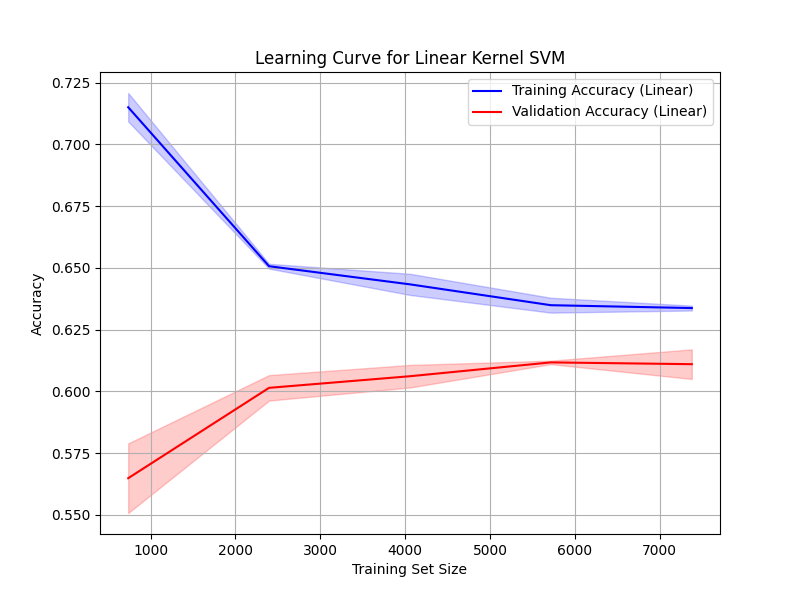
\includegraphics[width=\textwidth]{images/learning_curve_linear_SVM.png}
  \end{minipage}
  \begin{minipage}{0.45\textwidth}
      \centering
      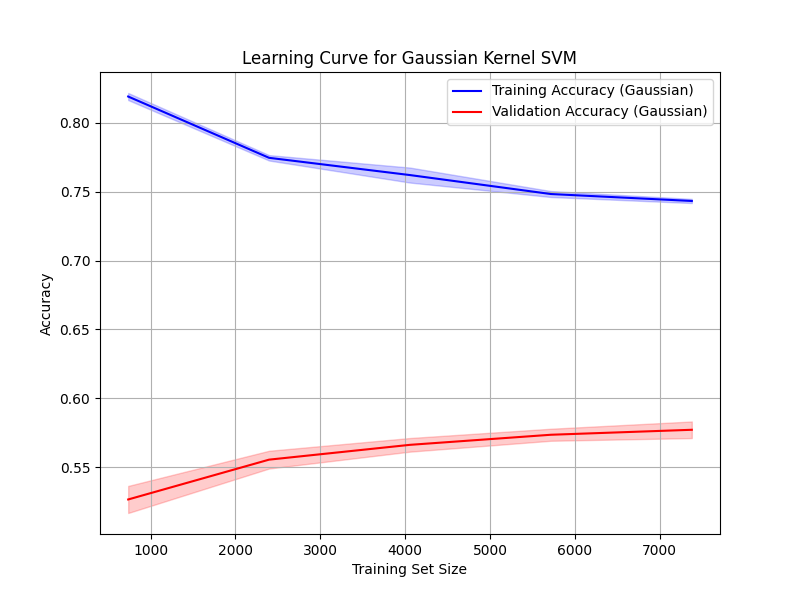
\includegraphics[width=\textwidth]{images/learning_curve_gaussian_SVM.png}
  \end{minipage}
\end{figure}

The learning curves for the linear and Gaussian kernel SVM models provide insights into their performance. The linear kernel SVM shows a consistent gap between the training and validation accuracy, indicating that the model may be underfitting the data. In contrast, the Gaussian kernel SVM exhibits a smaller gap, suggesting that it may be better suited to capturing the underlying patterns in the data. However, the slight decrease in validation accuracy with more training data in the Gaussian kernel SVM indicates that the model may still struggle with generalization to unseen data. Further adjustments to the model or feature engineering may be necessary to improve its performance.




\subsection{Random Forest}

\subsection{Neural Network}

\subsection{XGBoost}

\section{Result}

\section{Discussion}

\section{Reference}

\end{document}
